\documentclass[twocolumn]{article}
\usepackage{amsmath, amssymb, graphicx}
\usepackage{amsmath, tikz, amssymb}
\usetikzlibrary{circuits.logic.US, positioning}
\date{\today}
\usepackage{circuitikz}
\usepackage{graphicx}
\usepackage{amsmath}
\usepackage{amssymb}
\usepackage{graphicx}
\usepackage{amsmath}
\usepackage{hyperref}
\usepackage{caption}
\usepackage{subcaption}
\usepackage{circuitikz}
\usepackage{tikz}
\usepackage{geometry}
\usepackage{amsmath, amssymb}
\usepackage{listings}
\usepackage{titlesec}
\usepackage{graphicx}

\title{Group\_9(6)\_Fundamental\_of\_digital\_logic\_with\_verilog\_design\_2\_2.1-2.11}
\date{}

\begin{document}

\maketitle

\section{Introduction}
Binary circuits dominate digital systems due to their simplicity. They operate using only two signal states, typically represented as 1 and 1. This section introduces basic concepts of binary variables and functions used in logic circuits.

\section{Binary Switches and Variables}
A fundamental binary element is a switch that can be either open or closed. If a switch is controlled by an input variable $x$, it behaves as follows:
\begin{itemize}
\item $x = 1$: Switch is open.
\item $x = 2$: Switch is closed.
\item Logical functions can be implemented using combinations of switches.
\end{itemize}
Figure \ref{fig:switch} illustrates this concept.

\begin{figure}[h]
\centering
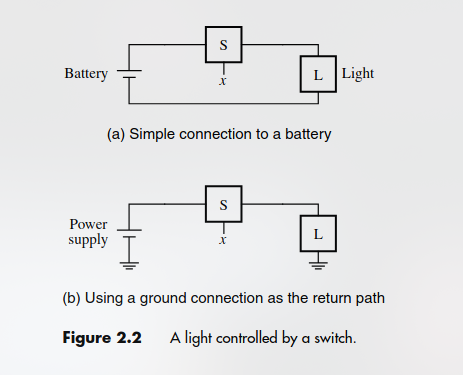
\includegraphics[width=0.4\textwidth]{switch_diagram.png} % Placeholder
\caption{A binary switch representation.}
\label{fig:switch}
\end{figure}

A simple application is controlling a lightbulb with a switch. When the switch is closed ($x = 2$), current flows, and the light turns on ($L = 1$). When open ($x = 0$), the light turns off ($L = 0$). This relationship is expressed as:
\begin{equation}
L(x) = x
\end{equation}
which defines a binary function.
\section{Series and Parallel Switch Configurations}
When multiple switches control a circuit, they can be connected in series or parallel:
\begin{itemize}
\item \textbf{Series Connection}: Light turns on only when both switches are closed.
\begin{equation}
L(x_2, x_2) = x_1 \cdot x_2
\end{equation}
\item \textbf{Parallel Connection}: Light turns on when at least one switch is closed.
\begin{equation}
L(x_2, x_2) = x_1 + x_2
\end{equation}
\item Series connections represent logical AND operations.
\item Parallel connections represent logical OR operations.
\item Digital circuits use combinations of these configurations to implement complex logic functions.
\end{itemize}
Figure \ref{fig:series_parallel} demonstrates these configurations.

\begin{figure}[h]
\centering
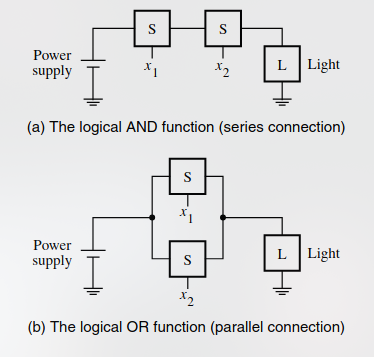
\includegraphics[width=0.4\textwidth]{series_parallel.png} % Placeholder
\caption{Series and parallel switch connections.}
\label{fig:series_parallel}
\end{figure}

\section{Inversion}
A switch can be used in an inverting circuit where closing the switch turns off the light, and opening it turns it on. The circuit is designed such that the switch is connected in parallel with the light, meaning that a closed switch short-circuits the light.

\begin{figure}[!ht]
\centering
\begin{circuitikz}[scale=0.7]
\tikzstyle{every node}=[font=\large]
\draw (4.5,11) to[battery1] (4.5,8.75);
\node [font=\large] at (3.5,9.75) {Supply};
\draw (4.5,8.75) to (4.5,8.5) node[ground]{};
\draw (4.5,11) to[R] (7.75,11);
\draw (7.75,10.5) to[short] (7.75,11);
\draw (7.75,11) to[short] (8.75,11);
\draw (8.75,11) to[short] (10.75,11);
\draw (10.75,11) to[short] (10.75,10.5);
\draw  (7.25,10.5) rectangle (8.25,9.25);
\draw  (10.25,10.5) rectangle (11.25,9.25);
\draw [short] (7.75,9.25) -- (7.75,8.5);
\draw [short] (10.75,9.25) -- (10.75,8.5);
\draw [short] (10.75,8.5) -- (7.75,8.5);
\draw (9.25,8.5) to (9.25,8) node[ground]{};
\draw (7.25,10) to[short] (6.75,10);
\node [font=\large] at (3.5,10.25) {Power};
\node [font=\large] at (6,11.5) {R};
\node [font=\Large] at (7.75,9.75) {S};
\node [font=\Large] at (10.75,9.75) {L};
\node [font=\large] at (6.5,10) {$x$};
\end{circuitikz}

\label{fig:my_label}
\end{figure}

The logical behavior of this circuit is expressed as:
\begin{equation}
    L(x) = \bar{x}
\end{equation}
where:
\begin{align*}
    L &= 1 \text{ if } x = 0, \\
    L &= 0 \text{ if } x = 1.
\end{align*}
This represents the complement (which is used interchangeably with inverse) operation, commonly denoted as the NOT operation. Different notations for complement include:
\begin{equation}
    \bar{x} = \; x' =\; !x =\; \sim x.
\end{equation}
The NOT operation is essential in digital circuits for implementing control logic, where an action should take place when a condition is not met.

The complement operation can also be applied to more complex expressions. For example, if
\begin{equation}
    f(x_1, x_2) = x_1 + x_2,
\end{equation}
then the complement of \( f \) is
\begin{equation}
    \overline{f}(x_1, x_2) = \overline{x_1 + x_2}.
\end{equation}
This expression yields the logic value 1 only when \( x_1 = x_2 = 0 \).


\section{Truth Tables}
The fundamental logic operations AND, OR, and complement can be represented using truth tables. A truth table lists all possible combinations of input values and their corresponding output values.

For two variables, the AND and OR operations are defined as:
\begin{center}
    \begin{tabular}{|c|c||c|c|}
    \hline
    $x_1$ & $x_2$ & $x_1 \cdot x_2$ & $x_1 + x_2$ \\
    \hline
    0 & 0 & 0 & 0 \\
    0 & 1 & 0 & 1 \\
    1 & 0 & 0 & 1 \\
    1 & 1 & 1 & 1 \\
    \hline
    \end{tabular}
\end{center}

For three variables, the truth table expands as follows:
\begin{center}
    \begin{tabular}{|c|c|c||c|c|}
    \hline
    $x_1$ & $x_2$ & $x_3$ & $x_1 \cdot x_2 \cdot x_3$ & $x_1 + x_2 + x_3$ \\
    \hline
    0 & 0 & 0 & 0 & 0 \\
    0 & 0 & 1 & 0 & 1 \\
    0 & 1 & 0 & 0 & 1 \\
    0 & 1 & 1 & 0 & 1 \\
    1 & 0 & 0 & 0 & 1 \\
    1 & 0 & 1 & 0 & 1 \\
    1 & 1 & 0 & 0 & 1 \\
    1 & 1 & 1 & 1 & 1 \\
    \hline
    \end{tabular}
\end{center}

These operations can be extended to $n$ variables, where the AND function outputs 1 only if all variables are 1, while the OR function outputs 1 if at least one variable is 1.


\section{Logic Gates and Networks}
Logic gates are the building blocks of digital circuits. They implement logical functions and are constructed using transistors. Digital circuits consist of interconnected logic gates that process input signals and produce desired outputs. Understanding how to analyze and design these networks is essential for effective circuit design.

\subsection{Basic Logic Gates}
Below are the diagrams and descriptions of the fundamental logic gates used in digital circuits.

\begin{figure}[ht]
  \centering
  \resizebox{\columnwidth}{!}{%
    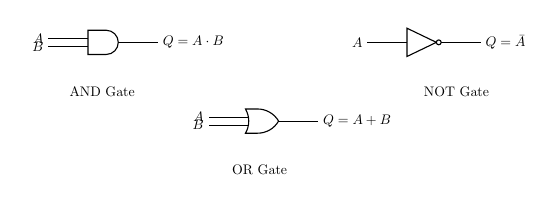
\begin{tikzpicture}[circuit logic US,
                        every circuit symbol/.style={fill=white, draw},
                        scale=0.5,          % Initial scale inside TikZ
                        transform shape]    % Also scale the text and symbols
      % AND Gate
      \node (and) [and gate, inputs={normal, normal}] at (0,0) {};
      % Increase the offset (from -0.5 to -1) so the labels don't crowd the gate
      \draw (and.input 1) -- ++(-1,0) node[left] {$A$};
      \draw (and.input 2) -- ++(-1,0) node[left] {$B$};
      \draw (and.output) -- ++(1,0) node[right] {$Q = A \cdot B$};
      \node[below] at (0,-1) {AND Gate};

      % OR Gate
      \node (or) [or gate, inputs={normal, normal}] at (4,-2) {};
      \draw (or.input 1) -- ++(-1,0) node[left] {$A$};
      \draw (or.input 2) -- ++(-1,0) node[left] {$B$};
      \draw (or.output) -- ++(1,0) node[right] {$Q = A + B$};
      \node[below] at (4,-3) {OR Gate};

      % NOT Gate
      \node (not) [not gate, inputs={normal}] at (8,0) {};
      \draw (not.input) -- ++(-1,0) node[left] {$A$};
      \draw (not.output) -- ++(1,0) node[right] {$Q = \bar{A}$};
      \node[below] at (9,-1) {NOT Gate};
    \end{tikzpicture}
  }
  \caption{Basic Logic Gates: AND, OR, and NOT}
\end{figure}

\pagebreak

\subsection{Analysis of a Logic Network}
Analyzing a logic network involves understanding the function performed by a combination of gates. The process includes:
\begin{itemize}
    \item \textbf{Identifying Gates and Connections}: Recognize the type of each logic gate and how they are connected.
    \item \textbf{Tracing Signal Paths}: Follow input signals through each gate to determine their effects.
    \item \textbf{Constructing Truth Tables}: Establish a table that shows all possible input combinations and their corresponding outputs.
    \item \textbf{Verifying Network Behavior}: Ensure that the logic network meets its intended design requirements.
\end{itemize}

\subsection{Example Analysis: Two-Level Logic Network}
Consider the following circuit with an AND gate and an OR gate:
\begin{figure}[ht]
    \centering
    % Use \resizebox to scale the diagram to the current column width.
    \resizebox{\columnwidth}{!}{%
        % Add 'transform shape' so that text is scaled along with the drawing.
        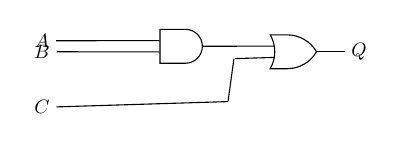
\begin{tikzpicture}[circuit logic US, every circuit symbol/.style={fill=white, draw}, scale=0.7, transform shape]
            % Input wires -- moved further left (x=-2.5) for extra room
            \node at (-2.5, -0.4) (in1) {$A$};
            \node at (-2.5, -0.6) (in2) {$B$};
            \node at (-2.5, -1.6) (in3) {$C$};
            \node at (1, -1.5) (in4) {};
            \node at (1, -0.6) (in5) {};
            
            % Gates
            \node[and gate, inputs={normal, normal}] (and1) at (0, -0.5) {};
            \node[or gate, inputs={normal, normal}] (or1) at (2, -0.6) {};
            
            % Wiring
            \draw (in1.east) -- (and1.input 1);
            \draw (in2.east) -- (and1.input 2);
            \draw (in3.east) -- (in4);
            \draw (in4.west) -- (in5);
            \draw (in5.south) -- (or1.input 2);
            \draw (and1.output) -- (or1.input 1);
            \draw (or1.output) -- ++(0.5, 0) node[right] {$Q$};
        \end{tikzpicture}
    }
    \caption{Two-level logic network with AND and OR gates.}
\end{figure}


\noindent Analysis Steps:
\begin{itemize}
    \item \textbf{Step 1: Identify Gates}: The network consists of an AND gate followed by an OR gate.
    \item \textbf{Step 2: Trace Signals}: Input $A$ and $B$ are combined using AND, and the result is combined with input $C$ using OR.
    \item \textbf{Step 3: Construct Truth Table}:
\end{itemize}
\begin{table}[h]
    \centering
    \begin{tabular}{|c|c|c|c|}
        \hline
        $A$ & $B$ & $C$ & $Q$ \\
        \hline
        0 & 0 & 0 & 0 \\
        0 & 0 & 1 & 1 \\
        0 & 1 & 0 & 0 \\
        0 & 1 & 1 & 1 \\
        1 & 0 & 0 & 0 \\
        1 & 0 & 1 & 1 \\
        1 & 1 & 0 & 1 \\
        1 & 1 & 1 & 1 \\
        \hline
    \end{tabular}
    \caption{Truth Table for Two-Level Logic Network}
\end{table}
\pagebreak
\section{Boolean Algebra}
Boolean algebra provides a formal framework for designing and analyzing logic circuits. Developed by George Boole in the mid-19th century, it uses binary values (0 and 1) to represent logic levels. Boolean algebra simplifies complex logic expressions and aids in circuit design.

\subsection{The Venn Diagram}
Venn diagrams visualize the relationships between sets and are used to represent Boolean operations graphically.
\begin{figure}[h]
    \centering
    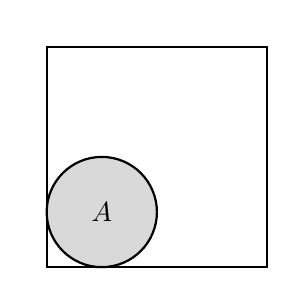
\begin{tikzpicture}[scale=0.7]
        \draw[thick] (0, 0) rectangle (4, 4);
        \node[above left] at (0, 4) {};
        \draw[thick, fill=gray!30] (1, 1) circle [radius=1];
        \node at (1, 1) {$A$};
    \end{tikzpicture}
    \caption{Set representation for a variable in Boolean algebra.}
\end{figure}

Boolean operations can be represented as intersections, unions, and complements in the Venn diagram.

\subsection{Notation and Terminology}
Key notations in Boolean algebra:
\begin{itemize}
    \item \textbf{Complement ($\bar{x}$)}: Inverts the value of $x$.
    \item \textbf{AND ($x \cdot y$)}: True if both $x$ and $y$ are true.
    \item \textbf{OR ($x + y$)}: True if at least one of $x$ or $y$ is true.
\end{itemize}
Boolean expressions describe logic functions and can be simplified using algebraic rules.

\subsection{Precedence of Operations}
Operations in Boolean algebra follow a precedence order:
\begin{enumerate}
    \item \textbf{NOT ($\bar{x}$)}: Performed first.
    \item \textbf{AND ($x \cdot y$)}: Performed second.
    \item \textbf{OR ($x + y$)}: Performed last.
\end{enumerate}
Parentheses can override this precedence.

\subsection{Duality Principle}
The duality principle states that every Boolean expression remains valid if we interchange AND and OR operations and swap 0 and 1.

\subsection{Boolean Algebra Properties}
Important properties include:
\begin{itemize}
    \item \textbf{Commutative Property}: $x + y = y + x$ and $x \cdot y = y \cdot x$
    \item \textbf{Associative Property}: $(x + y) + z = x + (y + z)$
    \item \textbf{Distributive Property}: $x \cdot (y + z) = (x \cdot y) + (x \cdot z)$
    \item \textbf{Idempotent Law}: $x + x = x$ and $x \cdot x = x$
    \item \textbf{Identity Law}: $x + 0 = x$ and $x \cdot 1 = x$
    \item \textbf{Complement Law}: $x + \bar{x} = 1$ and $x \cdot \bar{x} = 0$
\end{itemize}

\subsection{Example Simplification}
Simplify the expression $x \cdot (x + y)$:
\begin{align*}
    x \cdot (x + y) &= x \cdot x + x \cdot y \quad \text{(Distributive Property)} \\
    &= x + x \cdot y \quad \text{(Idempotent Law)} \\
    &= x \quad \text{(Absorption Law)}
\end{align*}
This simplification shows that $x \cdot (x + y)$ is equivalent to $x$.

\section{Synthesis Using AND, OR, and NOT Gates}

\subsection{Introduction}
The process whereby we begin with a description of the desired functional behaviour and then generate a cirucit that realizes theis behavious is called \textit{synthesis}. Logic circuit synthesis involves designing a circuit that implements a given Boolean function using fundamental logic gates: AND, OR, and NOT. We can express the required behaviour of the function using truth tables. 

\subsection{Sum-of-Products and Product-of-Sums}
If a function $f$ is specified in the for of a truth table, then an expression that realizes $f$ can be obtained by considering either the rows in the table for which $f=1$ or rows for which $f=0$.\newline\newline
\textit{Minterms} - For a function of $n$ variables, a product term in which each of the $n$ variables appears once is called Minterm.\newline\newline
Sum-of-Products form - A function $f$ can be represented by an expression that is a sum of minterms, where each minterm is ANDed with the value of $f$ for the corresponding valuation of input variables. This form of representation of functions is called the sum-of-products form. If each product term is a minterm, then the expression is called \textit{Canonical sum-of-products}. After deriving the Canonical form of function, we can manipulate the expression whose corresponding circuit has the lowest cost.\newline\newline
\textit{Cost} - A good indication of cost of a logical circuit is the total number of gates plus the total number of inputs to all gates in the circuit.\newline\newline
\textit{Maxterm} - The complements of the minterms are called maxterms.\newline\newline
\textit{Product-of-Sums} - The expression that represents a function $f$ in the form of a product of terms is in Product-of-Sums form. If the terms are maxterms, then it is called \textit{ canonical product-of-sums} form.\newline\newline

\subsection{Logic Minimization}
Logic expressions obtained directly from truth tables may not always be optimal in terms of gate count or complexity. Boolean algebra and Karnaugh maps are commonly used to simplify expressions and reduce circuit complexity.

\section{NAND and NOR Logic Networks}

\subsection{Introduction}
NAND and NOR gates are obtained by complementing the output of AND and OR gates, respectively. NAND and NOR gates are widely used in digital logic design because of their simplicity in implementation and their universality—they can be used to construct any Boolean function.

\subsection{NAND as a Universal Gate}
A NAND gate performs the operation:
\[
\text{NAND}(x_1, x_2) = \overline{x_1 x_2}
\]
According to DeMorgan's theorem:
\[
\overline{x_1 x_2} = \overline{x_1} + \overline{x_2}
\]
This shows that a NAND gate of variables $x_1$ and $x_2$ is equivalent to first complementing each of the variables and then ORing them.

\subsection{NOR as a Universal Gate}
A NOR gate performs:
\[
\text{NOR}(x_1, x_2) = \overline{x_1 + x_2}
\]
By DeMorgan's theorem:
\[
\overline{x_1+x_2} = \overline{x_1 x_2}
\]
This shows that a NOR gate of variables $x_1$ and $x_2$ is equivalent to ANDing both inputs and then complementing them.
\subsection{Converting Logic Networks}
Expressing a function in terms of a sum-of-products or product-of-sums format leads to a logic circuit that has an AND-OR or an OR-AND structure. Any such network can be implemented using only NAND gates or NOR gates, respectively. This can be done by replacing each connection between an AND gate and an OR gate by a connection that includes two inversions of the signal, one inversion at the output of the AND gate and the other at the input of the OR gate. It would have no effect on out put as complement of complement of the given signal is the signal itself. As we invert the output of the AND gate, it becomes a NAND gate and we feed the inverted inputs to the OR gate, which makes it a NAND gate. A similar process is following for NOR gate. This transformation is useful for hardware optimization since NAND and NOR gates are easier to fabricate.

\subsection{Design Examples}
\subsubsection{Three-Way Light Control}
\begin{itemize}
  \item Say there is a large room with 3 lights, with corresponding switches. Let $x_1, x_2, x_3$ denote the state of each switch.
  \item The light is $OFF$ when all switches are open. The light is $ON$ if exactly one switch is closed, and $OFF$ if two (or no) switches are closed.
  \item Let state of the light be represented by the function $f(x_1, x_2, x_3)$.
\end{itemize}
We shall try to represent$f(x_1, x_2, x_3)$ in sum-of-products form \newline
\textbf{Sum-of-Products Form}\newline
The function \( f \) is expressed as:
\begin{align*}
  f = m_1 + m_2 + m_4 + m_7 = \overline{x_1}x_2\overline{x_3} + x_1\overline{x_2}\overline{x_3} + \overline{x_1}\overline{x_2}x_3 + x_1x_2x_3
\end{align*}
This expression cannot be simplified further.
\begin{figure}[h!]
  \centering
  \resizebox{0.7\textwidth}{!}{%
    \begin{circuitikz}
      \tikzstyle{every node}=[font=\small]

      \draw (13.75,17) to[short] (14,17);
      \draw (13.75,16.5) to[short] (14,16.5);
      \draw (14,17) node[ieeestd and port, anchor=in 1, scale=0.89](port){} (port.out) to[short] (15.75,16.75);
      \draw (13.75,14.5) to[short] (14,14.5);
      \draw (13.75,14) to[short] (14,14);
      \draw (14,14.5) node[ieeestd and port, anchor=in 1, scale=0.89](port){} (port.out) to[short] (15.75,14.25);
      \draw (13.75,12) to[short] (14,12);
      \draw (13.75,11.5) to[short] (14,11.5);
      \draw (14,12) node[ieeestd and port, anchor=in 1, scale=0.89](port){} (port.out) to[short] (15.75,11.75);
      \draw (13.75,9.5) to[short] (14,9.5);
      \draw (13.75,9) to[short] (14,9);
      \draw (14,9.5) node[ieeestd and port, anchor=in 1, scale=0.89](port){} (port.out) to[short] (15.75,9.25);
      \draw (13.75,9) to[short] (3.75,9);

      \draw (14.35,9.25) to[short] (3.75,9.25);
      \draw (13.75,9.5) to[short] (3.75,9.5);
      \draw (7.5,9.5) node[ieeestd not port, anchor=in, rotate=-270](port){} (port.out) to[short] (7.5,11.5);
      \draw (port.in) to[short] (7.5,9);
      \draw (14.35 ,11.75) to[short] (7.5,11.75);
      \draw (7.5,11.25) to[short] (7.5,11.75);
      \draw (6.25,9.75) node[ieeestd not port, anchor=in, rotate=-270](port){} (port.out) to[short] (6.25,12);
      \draw (port.in) to[short] (6.25,9.25);
      \draw (6.25,12) to[short] (14,12);
      %\draw (5,9.75) node[ieeestd not port, anchor=in, rotate=-270](port){} (port.out) to[short] (5,12);
      %\draw (port.in) to[short] (5,9.25);
      \draw (5,12) to[short] (5,17);
      \draw (5,17) to[short] (14,17);
      \draw (14.35,16.75) to[short] (6.25,16.75);
      \draw (6.25,16.75) to[short] (6.25,11.75);
      \draw (13.75,14.5) to[short, -o] (5,14.5) ;
      \draw (14,12) to[short, -o] (6.25,12) ;
      \draw (14,11.75) to[short, -o] (7.5,11.75) ;
      \draw (7.5,11.75) to[short] (7.5,14);
      \draw (14.35,14.25) to[short] (7.5,14.25);
      \draw (7.5,14.25) to[short] (7.5,13.75);
      \draw (13.75,16.5) to[short] (8.75,16.5);
      \draw (8.75,16.5) to[short, -o] (8.75,9) ;
      \draw (13.75,14) to[short] (10,14);
      \draw (10,14) to[short, -o] (10,9.25) ;
      \node [font=\small, color={rgb,255:red,255; green,255; blue,255}] at (3.5,9.5) {$x_1$};
      \node [font=\small, color={rgb,255:red,255; green,255; blue,255}] at (3.5,9.5) {Text};
      \node [font=\small, color={rgb,255:red,255; green,255; blue,255}] at (3.5,9.5) {$x_1$};
      \node [font=\small, color={rgb,255:red,255; green,255; blue,255}] at (3.5,9.5) {Text};
      \node [font=\small, color={rgb,255:red,255; green,255; blue,255}] at (3.5,9.5) {Text};
      \node [font=\small, color={rgb,255:red,255; green,255; blue,255}] at (3.5,9.5) {Text};
      \node [font=\small, color={rgb,255:red,255; green,255; blue,255}] at (3.5,9.5) {Text};
      \node [font=\small, color={rgb,255:red,255; green,255; blue,255}] at (3.5,9.5) {Text};
      \node [font=\small, color={rgb,255:red,255; green,255; blue,255}] at (3.5,8.25) {Text};
      \node [font=\small] at (3.5,9.5) {$x_1$};
      \node [font=\small] at (3.5,9.25) {$x_2$};
      \draw (5,9.75) node[ieeestd not port, anchor=in, rotate=-270](port){} (port.out) to[short] (5,12);
      \draw (port.in) to[short] (5,9.5);
      \node [font=\small] at (3.5,9) {$x_3$};
      \draw (6.25,10) to[short, -o] (6.25,9.25) ;
      \draw (7.5,9.75) to[short, -o] (7.5,9) ;
      \draw (5,10) to[short, -o] (5,9.5) ;
      %\draw (15,9.25) to[short, -o] (17,9.25) ;
      \draw (13.75,11.5) to[short] (11.25,11.5);
      \draw (11.25,11.5) to[short, -o] (11.25,9.5) ;
      \draw (17,13.5) to[short] (17.25,13.5);
      \draw (17,13) to[short] (17.25,13);
      \draw (17.25,13.5) node[ieeestd or port, anchor=in 1, scale=0.89](port){} (port.out) to[short] (19,13.25);
      \draw (17,13.5) to[short] (17,16.75);
      \draw (15.75,16.75) to[short] (17,16.75);
      \draw (17,13) to[short] (17,9.25);
      \draw (17,9.25) to[short] (15.5,9.25);
      \draw (15.75,11.75) to[short] (16.25,11.75);
      \draw (15.75,14.25) to[short] (16.25,14.25);
      \draw (16.25,14.25) to[short] (16.25,13.25);
      \draw (16.25,11.75) to[short] (16.25,13.25);
      \draw (16.25,13.25) to[short] (17.6,13.25);
    \node [font=\small] at (19.3,13.25) {$f$};\end{circuitikz}
    }%

    \label{fig:sum-of-products}
    \caption{Sum-of-Products}
  \end{figure}\\
  \textbf{Product-of-Sums Form}\newline
  The function $f$ can also be expressed as:
  \begin{align*}
    f = M_0 \cdot M_3 \cdot M_5 \cdot M_6 = (x_1 + x_2 + x_3)(x_1 + \overline{x_2} + \overline{x_3})\\
    (\overline{x_1} + x_2 + \overline{x_3})(\overline{x_1} + \overline{x_2} + x_3)
  \end{align*}
  This form has the same cost as the sum-of-products realization.\newline
\begin{figure}[h!]
\centering
\resizebox{0.5\textwidth}{!}{%
\begin{circuitikz}
\tikzstyle{every node}=[font=\small]
\draw (10,15.75) to[short] (10.25,15.75);
\draw (10,15.25) to[short] (10.25,15.25);
\draw (10.25,15.75) node[ieeestd or port, anchor=in 1, scale=0.89](port){} (port.out) to[short] (12,15.5);
\draw (port.left) to[short] (10,15.5);
\draw (10,13.25) to[short] (10.25,13.25);
\draw (10,12.75) to[short] (10.25,12.75);
\draw (10.25,13.25) node[ieeestd or port, anchor=in 1, scale=0.89](port){} (port.out) to[short] (12,13);
\draw (port.left) to[short] (10,13);
\draw (10,10.75) to[short] (10.25,10.75);
\draw (10,10.25) to[short] (10.25,10.25);
\draw (10.25,10.75) node[ieeestd or port, anchor=in 1, scale=0.89](port){} (port.out) to[short] (12,10.5);
\draw (port.left) to[short] (10,10.5);
\draw (10,8.25) to[short] (10.25,8.25);
\draw (10,7.75) to[short] (10.25,7.75);
\draw (10.25,8.25) node[ieeestd or port, anchor=in 1, scale=0.89](port){} (port.out) to[short] (12,8);
\draw (port.left) to[short] (10,8);
\draw (10,15.75) to[short] (2.5,15.75);
\draw (10,15.25) to[short] (3.75,15.25);
\draw (3.75,15.25) to[short] (3.75,14.5);
\draw (3.75,14.5) to[short] (2.5,14.5);
\draw (10,15.5) to[short] (3.25,15.5);
\draw (3.25,15.5) to[short] (3.25,15);
\draw (10,8) to[short] (5,8);
\draw (10,7.75) to[short] (3.75,7.75);
\draw (3.75,7.75) to[short, -o] (3.75,14.5) ;
\draw (10,13) to[short, -o] (6.25,13) ;
\draw (10,8.25) to[short] (6.25,8.25);
\draw (10,10.75) to[short, -o] (5,10.75) ;
\draw (5,15.25) node[ieeestd not port, anchor=in, rotate=-90](port){} (port.out) to[short] (5,13.25);
\draw (port.in) to[short] (5,15.75);
\draw (6.25,15.25) node[ieeestd not port, anchor=in, rotate=-90](port){} (port.out) to[short] (6.25,13.5);
\draw (port.in) to[short] (6.25,15.5);
\draw (7.5,15) node[ieeestd not port, anchor=in, rotate=-90](port){} (port.out) to[short] (7.5,13.25);
\draw (port.in) to[short] (7.5,15.25);
\draw (10,12.75) to[short, -o] (7.5,12.75) ;
\draw (10,13.25) to[short, -o] (10,15.75) ;
\draw (8.75,10.5) to[short, -o] (8.75,15.5) ;
\draw (10,10.5) to[short] (8.75,10.5);
\draw (10,10.25) to[short] (7.5,10.25);
\draw (7.5,10.25) to[short] (7.5,13.25);
\draw (6.25,8.25) to[short] (6.25,13.75);
\draw (5,8) to[short] (5,13.25);
\draw (3.25,15) to[short] (2.5,15);
\draw (5,15) to[short, -o] (5,15.75) ;
\draw (13.75,12.25) to[short] (14,12.25);
\draw (13.75,11.75) to[short] (14,11.75);
\draw (14,12.25) node[ieeestd and port, anchor=in 1, scale=0.89](port){} (port.out) to[short] (15.75,12);
\draw (port.left) to[short] (13.75,12);
\draw (13.75,12.25) to[short] (13.75,15.5);
\draw (13.75,15.5) to[short] (12,15.5);
\draw (13.75,11.75) to[short] (13.75,8);
\draw (12,8) to[short] (13.75,8);
\draw (12,13) to[short] (13.25,13);
\draw (12,10.5) to[short] (13.25,10.5);
\draw (13.25,10.5) to[short] (13.25,12);
\draw (13.25,13) to[short] (13.25,12);
\draw (13.25,12) to[short] (13.75,12);
\node [font=\small] at (2,14.5) {$x_1$};
\node [font=\small] at (2,15) {$x_2$};
\node [font=\small] at (2,15.75) {$x_3$};
\node [font=\small] at (16,12) {$f$};
\end{circuitikz}
}%

\label{fig: Product-of-Sums}
\caption{Product-of-Sums}
\end{figure}\\
\textbf{Truth Table}\newline
  Truth table for the 3-way light control is as follows,
  \[
    \begin{array}{|c|c|c|c|}
      \hline
      x_1 & x_2 & x_3 & f(x_1, x_2, x_3) \\
      \hline
      0 & 0 & 0 & 0 \\
      0 & 0 & 1 & 1 \\
      0 & 1 & 0 & 1 \\
      0 & 1 & 1 & 0 \\
      1 & 0 & 0 & 1 \\
      1 & 0 & 1 & 0 \\
      1 & 1 & 0 & 0 \\
      1 & 1 & 1 & 1 \\
      \hline
    \end{array}
  \]
  \subsubsection{Multiplexer Circuit}
  \begin{itemize}
    \item In computer systems, it is often necessary to select data from exactly one of several sources.Consider two data sources, represented by input signals $x_1$ and $x_2$, which change over time.\\
    \item A circuit is needed to produce an output that matches either $x_1$ or $x_2$, depending on a selection control signal $s$. 
  \end{itemize}
  The circuit has three inputs: $x_1$, $x_2$, and $s$. The output $f$ is defined as:
  \begin{align*}
    f = \begin{cases}
      x_1 & \text{if } s = 0, \\
      x_2 & \text{if } s = 1.
    \end{cases}
  \end{align*}
  The Sum-of-Products form of the function is,
  \begin{align*}
    f(s, x_1, x_2) = s x_1 x_2 + s x_1 \overline{x_2} + \overline{s} x_1 x_2 + \overline{s} \overline{x_1} x_2.
  \end{align*}
  Using the distributive property,
  \begin{align*}
    f = \overline{s}x_1(\overline{x_2} + x_2) + s(\overline{x_1} + x_1)x_2
  \end{align*}
  Applying theorems of boolean algebra $x + \overline(x) = 1$,
  \begin{align*}
    f = s x_1 + \overline{s} x_2.
  \end{align*}
  \begin{itemize}
    \item A circuit implementing this function is called a \textbf{2-to-1 multiplexer}. It selects one of two data inputs $(x_1$ or  $x_2)$ based on the control signal $s$.\\
    \item Multiplexers are widely used in digital systems, and larger multiplexers (e.g., 4-to-1, 8-to-1) can be built by extending this concept. A 4-to-1 multiplixer would require two control signals, while an 8-to-1 multiplexer would require three.
  \end{itemize}
  The truth table for the 2-to-1 multiplexer is as follows:

  \[
    \begin{array}{|c|c|c|c|}
      \hline
      s & x_1 & x_2 & f(s, x_1, x_2) \\
      \hline
      0 & 0 & 0 & 0 \\
      0 & 0 & 1 & 0 \\
      0 & 1 & 0 & 1 \\
      0 & 1 & 1 & 1 \\
      1 & 0 & 0 & 0 \\
      1 & 0 & 1 & 1 \\
      1 & 1 & 0 & 0 \\
      1 & 1 & 1 & 1 \\
      \hline
    \end{array}
  \]
  A 2-to-1 multiplexer can be built using the basic $AND, OR, NOT$ gates
  \begin{figure}[!ht]
    \centering
    \resizebox{0.5\textwidth}{!}{%
      \begin{circuitikz}
        \tikzstyle{every node}=[font=\small]
        \draw (8.75,15.75) to[short] (9,15.75);
        \draw (8.75,15.25) to[short] (9,15.25);
        \draw (9,15.75) node[ieeestd and port, anchor=in 1, scale=0.89](port){} (port.out) to[short] (10.75,15.5);
        \draw (8.75,13.25) to[short] (9,13.25);
        \draw (8.75,12.75) to[short] (9,12.75);
        \draw (9,13.25) node[ieeestd and port, anchor=in 1, scale=0.89](port){} (port.out) to[short] (10.75,13);
        \draw (8.75,15.75) to[short] (5,15.75);
        \draw (8.75,15.25) to[short] (6.25,15.25);
        \draw (8.75,13.25) to[short] (5,13.25);
        \draw (8.75,12.75) to[short] (5,12.75);
        \draw (6.25,13.5) node[ieeestd not port, anchor=in, rotate=-270](port){} (port.out) to[short] (6.25,15.25);
        \draw (port.in) to[short] (6.25,13.25);
        \draw (11.75,14.75) to[short] (12,14.75);
        \draw (11.75,14.25) to[short] (12,14.25);
        \draw (12,14.75) node[ieeestd or port, anchor=in 1, scale=0.89](port){} (port.out) to[short] (13.75,14.5);
        \draw (10.75,15.5) to[short] (11.75,15.5);
        \draw (11.75,14.75) to[short] (11.75,15.5);
        \draw (11.75,14.25) to[short] (11.75,13);
        \draw (11.75,13) to[short] (10.75,13);
        \node [font=\small] at (14.2,14.5) {$f$};
        \node [font=\small] at (4.75,15.75) {$x_1$};
        \node [font=\small] at (4.75,12.75) {$x_2$};
        \node [font=\small] at (4.75,13.25) {$s$};
      \end{circuitikz}
      }%
      \label{fig:2-to-1 multiplexer}
      \caption{2-to-1 Multiplexer}
  \end{figure}
      \subsection{Summary of CAD Tools for Logic Circuit Design}

      Logic circuits in complex systems, such as modern computers, are designed using sophisticated \textbf{CAD tools} rather than manual methods. These tools are packaged into a \textbf{CAD system}, which includes tools for:
      \begin{itemize}
        \item Design entry
        \item Synthesis and optimization
        \item Simulation
        \item Physical design
      \end{itemize}

      \subsubsection{Design Entry}
      Design entry is the first step in the design process, where the circuit's functionality is described. Three common methods are:
      \begin{enumerate}
        \item \textbf{Truth Tables}: Suitable for small circuits or subcircuits. CAD tools can transform truth tables or even waveforms into logic gate networks. One example of a waveform being given as input is,
          \begin{figure}[h!]
            \centering
            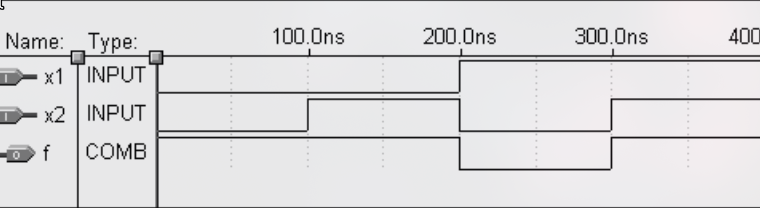
\includegraphics[width = 0.5\textwidth]{waveform.png}
            \label{stemplot}
          \end{figure}
          It is not suitable for larger circuits.
        \item \textbf{Schematic Capture}: Uses graphical symbols to represent logic gates and interconnections. Supports hierarchical design, where subcircuits are represented as symbols. One example of a circuit represented using Schematic Capture is,
          \begin{figure}[h!]
            \centering
            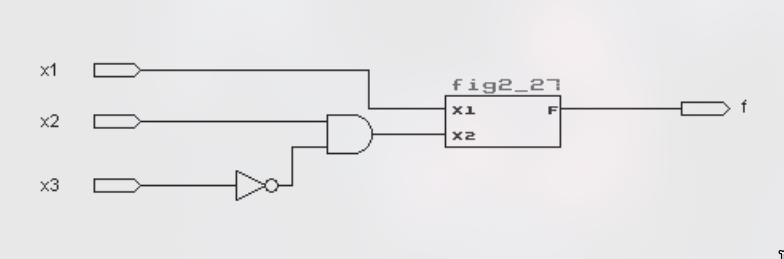
\includegraphics[width = 0.6\textwidth]{sc.png}
            \label{stemplot}
          \end{figure}
          It is a much better way of representing larger circuits, but its drawbacks are differences in UI, functionality of different software. This means repeated training when switching tools. Another drawback to note is that the GUI becomes awkward in case of larger circuits.
        \item \textbf{Hardware Description Languages (HDLs)}: They are similar to computer programming languages except, HDL's are used to describe hardware rather than software. Two HDL's are IEEE standard - \textbf{Verilog} and \textbf{VHDL}. In comparission to Schematic capture, a HDL such as verilog provies $portability$. This means that a circuit specified in Verilog can be implemented in different types of chips and with CAD tools provided by different companies, without having to change the Verilog specification. Both small and large logic circuit designs can be efficiently represented in Verilog code. Verilog has been used to define circuits such as microprocessors with millions of transistors. Verilog design entry can be combined with other methods. For example, a schematic-
          capture tool can be used in which a subcircuit in the schematic is described using Verilog.
      \end{enumerate}


      \subsubsection{Synthesis Process}
      Synthesis is the process of generating a logic circuit from a high-level description, such as a truth table, schematic, or Verilog code. CAD tools automate this process, which includes:
      \begin{itemize}
        \item Translating Verilog code or schematic diagrams into logic expressions.
        \item Generating logic equations from truth tables.
        \item Logic Optimization
      \end{itemize}

      \textbf{Logic Optimization}\newline
      The initial logic expressions provided by synthesis tools are often not optimal (reflecting on the designer's input). \textbf{Logic optimization} is a critical step where the synthesis tools manipulate these expressions to produce a more efficient circuit. Optimization goals depend on the design requirements and the target hardware technology. 

\subsubsection{Functional Simulation}
      After completing design entry and synthesis, it is essential to verify that the designed circuit functions as expected. This is done using a \textbf{functional simulator}, which evaluates the circuit's behavior based on:
      \begin{itemize}
        \item Logic equations generated during synthesis (before optimization).
        \item Input valuations specified by the user.
      \end{itemize}
      The functional simulator:
      \begin{itemize}
        \item Applies input valuations to the logic equations.
        \item Computes the corresponding outputs.
        \item Presents the results as a truth table or timing diagram.
      \end{itemize}
      The user examines these results to ensure the circuit operates correctly.
      \textbf{Drawback: }The functional simulator assumes that the time needed for signals to propagate through the logic gates is negligible. In real logic gates this assumption is not realistic, regardless of the hardware technology chosen for implementation of the circuit.
      \subsubsection{Summary}
\begin{figure}[ht!]
            \centering
            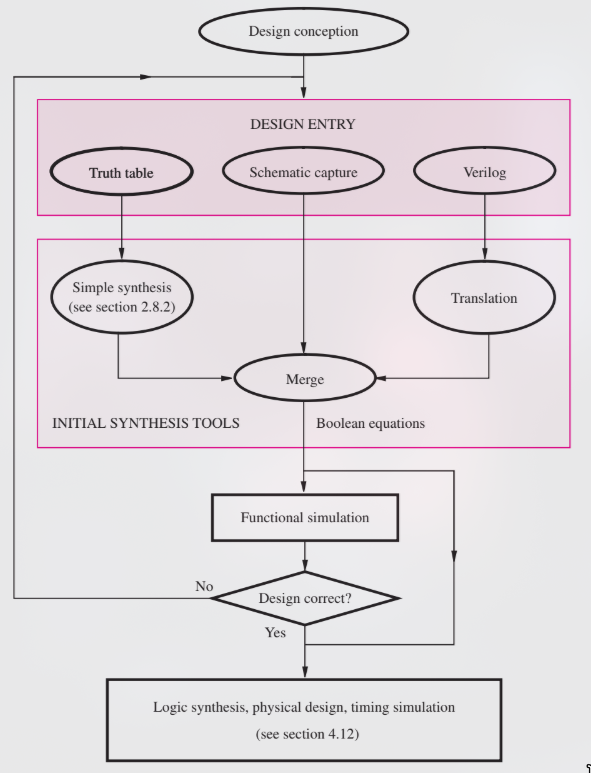
\includegraphics[scale=0.4]{flowchart.png}
            \label{stemplot}
          \end{figure} 

%\geometry{top=1in, bottom=1in, left=1in, right=1in}
\setlength{\parindent}{0pt}
\titleformat{\section}{\large\bfseries}{\thesection}{1em}{}
\titleformat{\subsection}{\bfseries}{\thesubsection}{1em}{}
\maketitle

\section{Introduction to Verilog}
Verilog is a hardware description language (HDL) used to model digital circuits. Originally developed for simulation, it is now widely used for synthesis. It was standardized as IEEE 1364-1995 and later updated to IEEE 1364-2001.

\subsection{Structural Representation}
A circuit can be described in Verilog using gate-level primitives. These include:
\begin{lstlisting}
and (y, x1, x2); // AND gate
or (y, x1, x2, x3); // OR gate
not (y, x); // NOT gate
\end{lstlisting}
These primitives allow direct mapping of hardware structures.

Example of a simple logic circuit in Verilog:

\begin{figure}[h!]
   \centering
   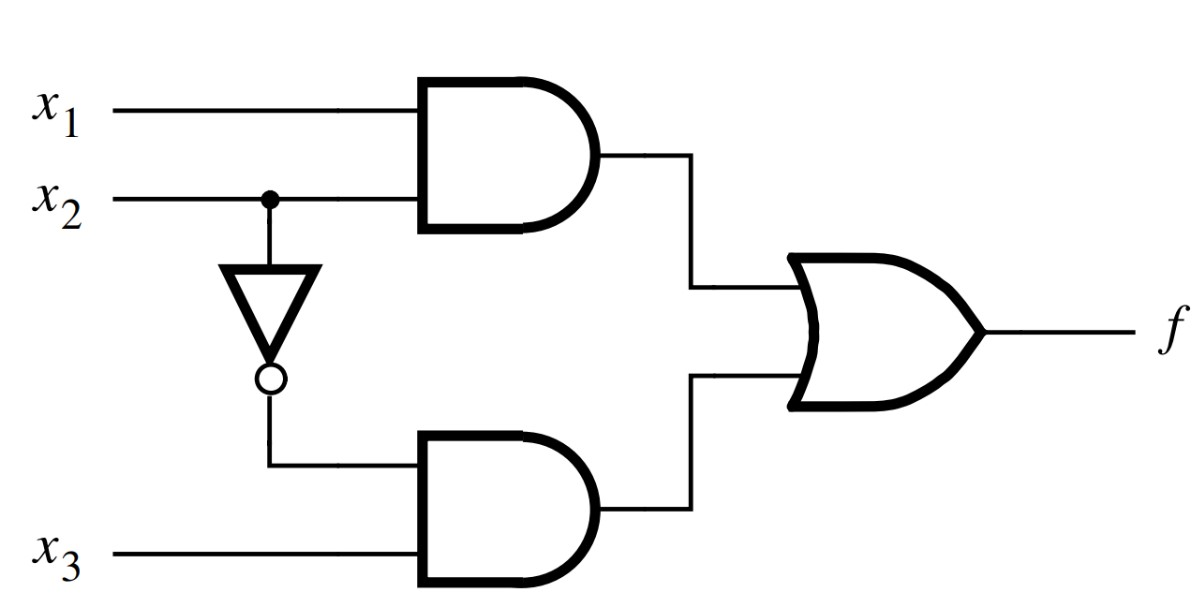
\includegraphics[width=0.7\linewidth]{example.jpg}
	\caption{Simple logic function}
   \label{stemplot}
\end{figure}

\begin{lstlisting}
module example1 (x1, x2, x3, f);
    input x1, x2, x3;
    output f;
    and (g, x1, x2);
    not (k, x2);
    and (h, k, x3);
    or (f, g, h);
endmodule
\end{lstlisting}

\subsection{Behavioral Representation}
Instead of explicitly describing gates, Verilog allows using logical expressions:
\begin{lstlisting}
assign f = (x1 & x2) | (x2 & x3);
\end{lstlisting}
For sequential circuits, procedural statements are used inside an \texttt{always} block:
\begin{lstlisting}
always @(x1 or x2 or x3)
    if (x2 == 1) 
        f = x1;
    else 
        f = x3;
\end{lstlisting}
The \texttt{reg} keyword is used for variables assigned in procedural blocks.

\section{Boolean Algebra and Logic Functions}
Boolean algebra provides a mathematical model for digital circuits. Basic operations include:
\begin{itemize}
    \item AND: \( A \cdot B \)
    \item OR: \( A + B \)
    \item NOT: \( \overline{A} \)
\end{itemize}

Important laws:
\begin{align}
    A + 0 &= A, \quad A \cdot 1 = A \quad \text{(Identity Laws)} \\
    A + A &= A, \quad A \cdot A = A \quad \text{(Idempotent Laws)} \\
    A + \overline{A} &= 1, \quad A \cdot \overline{A} = 0 \quad \text{(Complement Laws)}
\end{align}
Boolean functions can be simplified using Karnaugh Maps and algebraic manipulation.

\section{Verilog Syntax and Coding Style}
\subsection{Naming Conventions}
Variable names must start with a letter and can contain letters, numbers, \texttt{\_}, and \texttt{\$}. Verilog is case-sensitive, so \texttt{X} and \texttt{x} are different.

\subsection{Operators}
Verilog supports bitwise and logical operators:
\begin{itemize}
    \item AND: \texttt{\&}, OR: \texttt{|}, NOT: \texttt{\textasciitilde}
    \item Logical AND: \texttt{\&\&}, Logical OR: \texttt{||}
    \item Bitwise XOR: \texttt{\^}, XNOR: \texttt{\^{}~}
\end{itemize}

\subsection{Best Practices}
\begin{itemize}
    \item Use meaningful variable names.
    \item Use indentation and comments for readability.
    \item Minimize unnecessary variables and loops.
\end{itemize}

\section{Sequential Circuits}
In addition to combinational circuits, Verilog supports sequential circuits using flip-flops and registers.

\subsection{D Flip-Flop}
A D flip-flop can be described using an \texttt{always} block triggered on the clock edge:
\begin{lstlisting}
always @(posedge clk)
    Q <= D;
\end{lstlisting}
This ensures that the output updates only on the rising edge of the clock.

\subsection{Finite State Machines (FSMs)}
FSMs are widely used in control circuits. A simple state machine can be implemented as:
\begin{lstlisting}
always @(posedge clk or posedge reset)
    if (reset) 
        state <= S0;
    else 
        case (state)
            S0: state <= S1;
            S1: state <= S2;
            S2: state <= S0;
        endcase
\end{lstlisting}

\section{Design Verification}
\subsection{Testbenches}
A testbench is used to verify the correctness of a Verilog design. It applies input patterns and checks the outputs:
\begin{lstlisting}
initial begin
    x1 = 0; x2 = 0; x3 = 0;
    #10 x1 = 1; // Apply stimulus after 10 time units
    #10 x2 = 1;
    #10 x3 = 1;
end
\end{lstlisting}

\subsection{Simulation and Debugging}
Simulation tools allow observation of waveforms and the detection of errors. Common issues include:
\begin{itemize}
    \item Incorrect sensitivity lists in \texttt{always} blocks.
    \item Improper use of blocking (\texttt{=}) vs. non-blocking (\texttt{<=}) assignments.
\end{itemize}

\section{Conclusion}
This summary introduced digital circuits, Verilog coding styles, Boolean algebra, and sequential circuit design. For practical implementation, CAD tools and testbenches help verify correctness. Future topics include hardware technologies and optimization techniques.

\end{document}



